\section{Theory}
\label{sec:Theorie}

\subsection{Diode laser}

A Diode laser is used in the experiment.
In principle the laser consists of three main parts.
\begin{itemize}
    \item An active medium
    \item A pump
    \item A resonator
\end{itemize}
The \textbf{active medium} consists of a \textbf{p-type} and an \textbf{n-type} semiconductor.
A semiconductor has a conductivity that falls between that of an insulator and a conductor.
This property can be explained by the band model. 
As a result of the crystal structure of condensed matter all of the atoms in the crystal are very close together which would mean that their electrons would share the same quantum state.
The Pauli exclusion principle forbids this so the energy state of the electrons slightly change.
The result is the so-called electronic band structure.
This means that a lot of energy levels are almost the same, these energy levels can be discribed as one band.
After one band there is a band gap in which no possible energy levels lie after the gap next band starts.
\\\\
The highest band that's still occupied by electrons at the Fermi level, which is at absolute zero temperature, is called the valence band.
The conduction band is the band that follows the valence band.
In metals the properties of those two bands are combined, because the Fermi energy lies inside a band as shown in Figure \ref{fig:band_structure}.

\begin{figure}
    \centering
    \caption{The band structure of different types of condensed matter, the shades follow the Fermi-Dirac distrubution of the electrons in the given material. The Figure is taken from source \cite{wikipedia_valence_conduction_band}}
    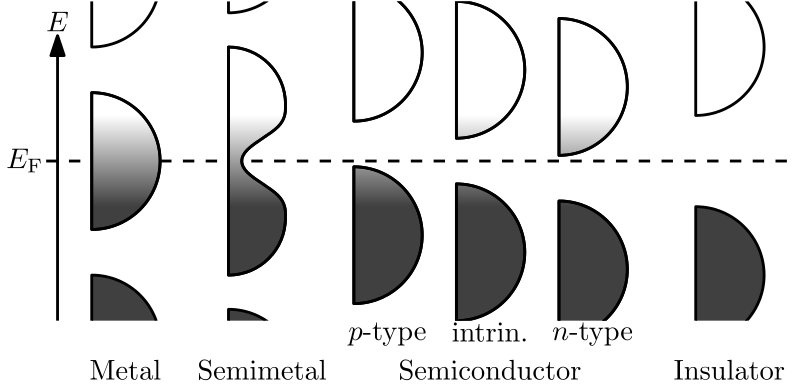
\includegraphics[width=0.75\textwidth]{content/data/Band_structure_diffrent_materials.png}
    \label{fig:band_structure}
\end{figure}

In semiconductors those bands are distinc from another so the conduction band lies above the Fermi level and the valence band beneath.
This means at absolute zero the semiconductor does not conduct.
With rising temperature more electrons move from the valence band into the conduction band so the semiconductor gains the property to conduct.
This property alone is not usefull on it's own for building a laser.
To modify the conductivity and properties of the semiconductor, impurities get introduced into the crystal lattice.
Depending on the material used the result is called a p-type or n-type semiconductor.
This process is called doping.
\\\\
\FloatBarrier
For a \textbf{p-type} semiconductor an impurity is used that has less valence electrons than the material that builds the semiconductor crystal.
This way an electron hole is created, which behaves like a missing charge which can freely move through the crystal.
The missing charge has the properties of a positiv charge.
A picture visualizing the p-type doping is shown in Figure \ref{fig:p-type_doping}.
As seen in the picture the Boron has one less valence electron so it can not form a covalent bond with the silicon on it's right.
This results in a missing charge that can move through the crystal.
\begin{figure}
    \caption{Through different doping materials it's possible to achieve p-type and n-type semiconductors, as shown in the pictures.}
    \begin{subfigure}{0.48\textwidth}
        \centering
        \caption{A two dimensional scheme, of a p-type semiconductor made of silicon, doped with Boron. The picture is taken from source \cite{p-type_doping}.}
        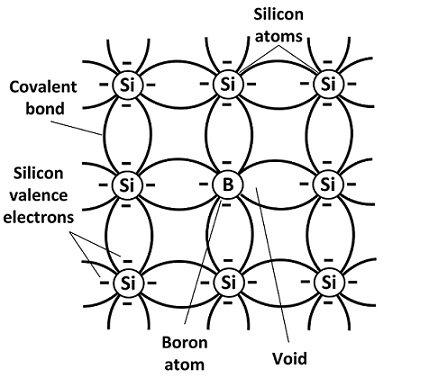
\includegraphics[height=5cm]{content/data/p-type-semiconductor-doping.jpg}
    \label{fig:p-type_doping}
    \end{subfigure}
    \hfill
    \begin{subfigure}{0.48\textwidth}
        \centering
        \caption{A two dimensional scheme, of an n-type semiconductor made of silicon, doped with Antimony. The picture is taken from source \cite{p-type_doping}.}
        \includegraphics[height=5cm]{content/data/N-Type-semiconductor-doping.jpg}
        \label{fig:n-type_doping}
    \end{subfigure}
    \label{fig:p-n-type_doping}
\end{figure}
Doping is also possible with an impurity that has more valence electrons than the crystal material.
In that case the electron that can not form a covalent bond is able to move freely through the crystal.
The result is a free negativ charge. In this case the semiconductor is called an \textbf{n-type} semiconductor.
The picture \ref{fig:n-type_doping} shows an n-type semiconductor made of silicon which is doped with antimony.
The result is a fith valence electron that can not form a valence bond and in return is able to move trough the crystal.
\\\\
\FloatBarrier
If now a p-type and an n-tpye semiconductors are brought together the free electrons from the n-type semiconductor tend to move into the holes of the p-type semiconductor.
This results in the emission of photons, because the energy of the n-type electrons is higher than the energy states in which they drop in the p-type semiconductor.
This process is used as active medium in the diode laser.
\\\\
But the active medium alone is not of much use, because the flow of electrons from n-type to p-type stops after a short while.
This is because an equilibrium forms.
To keep the electrons moving they have to be brought back into the n-type semiconductor.
So they have to be pumped up into the higher energy state they had before they moved into to the p-type semiconductor.
The \textbf{pump} is made by applying an electric field to both semiconductor layers.
With the electric field the electrons are injected into the n-type semiconductor to start the cycle over again.
\\\\
With the pump and the active medium alone the laser would already emit light but that light is not coherent, so the basic property of laser light is still missing.
To make the laser just emit coherent light a resonator is needed.
\\\\
A \textbf{resonator} consists of two reflective layers that engulf the active medium.
The distance $L$ between those mirrors is choosen to be $n \lambda/2 = L$ with $n$ as natural number, $\lambda$ the wavelength of the laser light.
This way, whenever light gets emited by the active medium it's trapped between the reflective layers and forms a standing wave.
The photons than bounce back and forth in the resonator and provide a feedback for the active medium.
Which results in the emission of more photons with the same characteristics as the initial photons.
In the Diodelaser the resonator consists of a cavity that is made by two cleaved facets at the ends of the diode chip.
Depending on the coating of these the reflectivity increases or decreases.
Usually one of the mirrors completly reflects the photons and the other mirror lets some photons pass through.
This way the light emitted by the laser consists of the photons that pass through the mirror.
\\\\
With all these components the Diodelaser emits laser light with a wavelength near $\lambda = \SI{785}{\nano\meter}$, with an output power of about $P_\text{laser} = \SI{70}{\milli\W}$.

\subsection{Diffraction Grating}
Bare Diodelasers emit light with a large bandwith $\Delta f_\text{laser} = \SI{50}{\mega\Hz}$, which is large compared to the linewidths of atomic transitions $\Delta f_\text{atomic} = \SI{5}{\mega\Hz}$.
They are also very sesitive to optical feedback, so it's not desirable to reflect any light back into the internal laser cavity.
To solve this problem a Diffraction Grating is installed in front of the laser, as shown in Figure \ref{fig:grating}.

\begin{figure}
    \centering
    \caption{A grating is installed in front of the laser to prevent outside feedback as well as shortening the bandwidth of the laserlight. The Figure is taken from source \cite[5]{anleitung_laser}}
    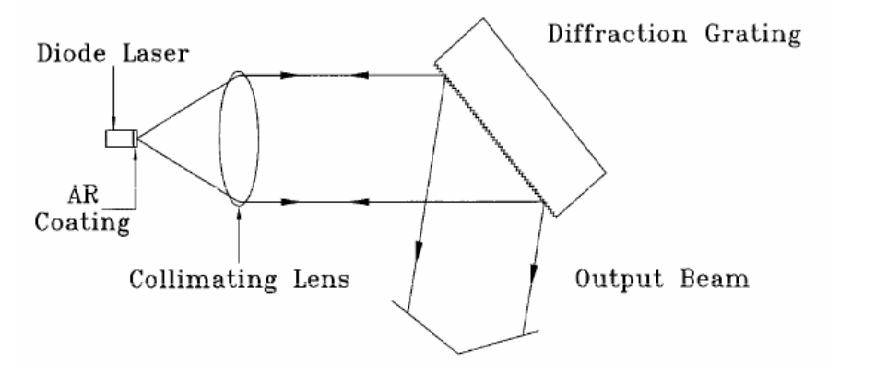
\includegraphics[width=0.75\textwidth]{content/data/grating.png}
    \label{fig:grating}
\end{figure}

About $85\%$ of the light that hits the grating gets reflected, this light has grating order $m=0$.
The other $15\%$ are reflected back into the laser to form an external cavity.
The light that's reflected back into the laser is of grating order $m=1$.
Light that travels back into the laser stabilizies the frequency of the laser and narrows the linewidth to less than $\Delta f_\text{laser} = \SI{1}{\mega\Hz}$.


\subsection{Laser tuning}
Because the laser always tends to lase in the frequency with the greatest net gain we want to find that frequency.
This frequency depends on four factors:
\begin{itemize}
    \item The medium
    \item The internal cavity
    \item The Grating Feedback
    \item The External cavity.
\end{itemize}
All these factors have an influence on the net gain and with that on frequency of the laser.
The different influences are shown in Figure \ref{fig:netgain}.
\begin{figure}
    \centering
    \caption{The net gain of every components should peak at the wavelength $\lambda_0$, the net gain of every component is shown in this picture. The picture is taken from source \cite[6]{anleitung_laser}.}
    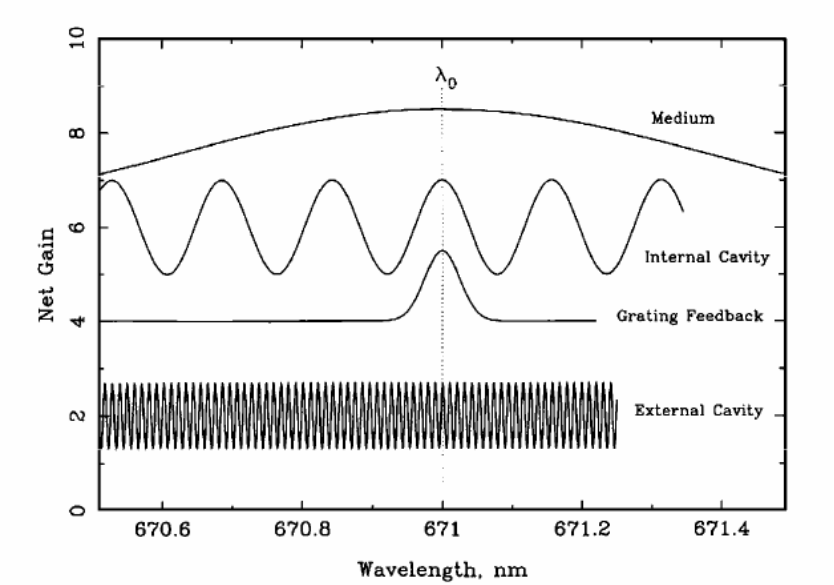
\includegraphics[width=0.75\textwidth]{content/data/netgain.png}
    \label{fig:netgain}
\end{figure}
\FloatBarrier
\subsubsection{Medium gain}
The medium gain depends on the properties of the semiconductor and also depends on the temperature of the laser.
But because the temperature of the laser will be determined in the experiment we can assume that the medium lases with a wavelength of about $\SI{785}{\nano\meter}$ as mentioned before.

\subsubsection{Internal cavity gain}
The internal cavity adds an influence onto the frequency of the laser.
It's net gain is frequency dependent, as shown in figure \ref{fig:netgain}.
The period is defined by the length of the cavity $L$, the index of refraction $n$, the speed of light $c$ and is given by
$\Delta f_\text{int} = \frac{c}{2Ln}$.

\subsubsection{Grating gain}
The grating can be shifted.
That way only the light from a narrow wavelength band will be fed back into the cavity.
The light wavelength can be found by the Bragg condition $\lambda = \frac{2d \sin{\theta}}{n}$ with the grid spacing $d$, the diffraction order $n$ and the glancing angle $\theta$.
Because the diffraction order $n = 1$, we can write the Bragg condition as $\lambda = 2d\sin{\theta}$.
With this the $\Delta f$ is given by $\frac{f}{\Delta f} = N$ with $N$ as the number of grating lines, subtended by the laser beam.
In the experiment $N=5400$ which results into $\Delta f \approx \SI{70}{\giga\Hz}$.

\subsubsection{External cavity gain}
The external cavity is made by the grating and the back facet of the diode.
Similar to the internal cavity it's net gain also periodicly shifts, with $\Delta f = \frac{c}{2L}$.
\\
But the distance is larger than that of the internal cavity which results to $\Delta f_\text{ext} \approx \SI{10}{\giga\Hz}$.
Because the period is dependent on the distance between the grating and the diode the period also changed when the grating is moved.
\\\\
Forcing the laser into lasing with a single mode is achieved by changing the net gain of every component discussed before to the wavelength $\lambda_0$ of the medium.
The optimal case is pictured in Figure \ref{fig:netgain}, as every net gain peaks at $\lambda_0$.

\subsection{Absorption from Rubidium}
Photons have the ability to raise the energy state of electrons in atoms.
After some time the electron falls back to its initial state and emits light with the frequency/wavelength as the photon that started the process.
The electron can also move back into its initial state by falling back in multiple steps.
This realises multiple photons doing so, the sum of energy of the released photons must be the same.
The material that absorbs light in this experiment is Rubidium more specific $\ce{^{85}Rb}$ and $\ce{^{87}Rb}$.
There Absorption spectrum lies with in the wavelength of the laser used in the experminet.